\documentclass[10pt,a4paper,twoside]{article}
\usepackage[utf8]{inputenc}
\usepackage{amsmath}
\usepackage{amsfonts}
\usepackage{amssymb}
\usepackage{graphicx}
\usepackage[margin=1in]{geometry}
\author{Nathan Cunningham}
\title{Progress to date: 13/07/2016}
\begin{document}
\maketitle
\section{Read paper: Bayesian cluster analysis: point estimation \& credibles balls by Wade \& Ghahramani}
Summary:
\begin{itemize}
\item Paper\cite{wade2015bayesian} deals with the problem of summarising the output of a bayesian nonparametric cluster analysis. These analyses provide a posterior over the entire space of clusterings although typically a point estimate along with an associated measure of uncertainty are of interest.
\item The authors consider an information and decision theoretic techniques for summarising the posterior clustering allocations via the construction of a loss function:
\begin{equation}
c^{*} = argmin_{\hat{c}} \Sigma_{c} \mathbb{L}(c, \hat{c}) p(c|y_{1:N})
\end{equation}
which is a loss associated with approximating the true cluster allocation, c, by an allocation $\hat{c}$ averaged over all possible clusterings.
\item Loss functions should satisfy some basic principles such as invariance to permutations of data points indices or cluster labels.

\item They first present Binder's loss which penalises for (1) assigning pairs to the same cluster when they should be in different clusters and (2) assigning pairs to different clusters which should be in the same cluster. This is similar to the Rand Index which considers concordance across cluster allocations, whereas this considers discordance across cluster allocations.
\item The authors proposal is to use the variation of information (VI) as the loss function. VI compares information within two clusterings with information shared between them. Their proposed loss function is:
\begin{equation}
2H(c, \hat{c}) - H(c) - H(\hat{c})
\end{equation}
where $H(c)$ is the information contained in cluster allocation c, while $H(c, \hat{c}$ is the information contained in each allocation, removing the shared information.

\begin{equation}
\sum_{i = 1}^{k_N} \frac{n_{i+}}{N}log\left(\frac{n_{i+}}{N}\right) + 
\sum_{j = 1}^{\hat{k}_N} \frac{n_{+j}}{N}log\left(\frac{n_{+j}}{N}\right) -
2 \sum_{i = 1}^{k_N}\sum_{j = 1}^{\hat{k}_N} \frac{n_{ij}}{N}log\left(\frac{n_{ij}}{N}\right)
\end{equation}

\item A comparison is made of VI and the Binder loss. They are each metrics on the partition space, satisfying non-negativity, symmetry and the triangle inequality. Binder's loss tends to favour splitting clusters rather than merging which can lead to large numbers of clusters.

\item Due to impossibility of comparing losses across \textit{all} luster allocations, suggest a greedy search algorithm:
\begin{itemize}
\item Initialise $\hat{c}$
\item For i = 1, ...,
\begin{itemize}
\item Find the l closest partitions that cover $\hat{c}$, and the l closest partitions that $\hat{c}$ covers.
\item Compute $\mathbb{E}\left[L(c, \hat{c} | \mathbb{D}\right]$ for all 2l partitions and select the partition, $c^{*}$, which minimises this
\item If the expected loss for $c^{*}$ is less than for $\hat{c}$, set $\hat{c} = c^{*}$, otherwise stop
\end{itemize}

\end{itemize}

\item This also allows for specification of a 'ball' of size $\epsilon$ around a clustering:
\begin{equation}
\mathbb{B}_{\epsilon}(\hat{c}) = {c: d(\hat{c}, c) \leq \epsilon} 
\end{equation}

\end{itemize}

Use:
\begin{itemize}
\item The original SMC clustering algorithm outputs a separate clustering allocation for each of the particles. Feeding forward into the MDI algorithm would require selection of an optimal allocation. This may be useful.
\item May also be useful within the context of deciding the final allocation for the MDI.
\end{itemize}

\section{Integration of MDI and SMC clustering code}
\begin{itemize}
\item Implementing SMC clustering methods within the MDI.
\item Involves the modification of the \texttt{DrawNewItemLabel} function in MDI:
\begin{itemize}
\item Originally MDI involves upweighting the allocation probabilities to account for the concordance across datasets. Then considers the allocation of each data point to each of the occupied clusters and one unoccupied cluster and assigns to the cluster best supported by the data. Replace the step with allocating to each cluster with the SMC step.
\item Results at this stage are not promising, (Figure \ref{fig:alloc}). Algorithm appears to assign most observations to the same cluster, differing from the previous output of the MDI algorithm.
\item Still a lot to do with integrating the code. 
\begin{itemize}
\item It currently only runs using a single particle, meaning that particle is the one that gets accepted. Need to work on selecting a particular cluster from the particle filter run.
\item Currently begins fresh every run of the algorithm, no parameters carried across.
\item The parameters from the gamma matrix are not being used correctly.
\item Many wasteful calculations being carried out as remnants of the previous algorithm.
\end{itemize}
\end{itemize}
\end{itemize}

\begin{figure}
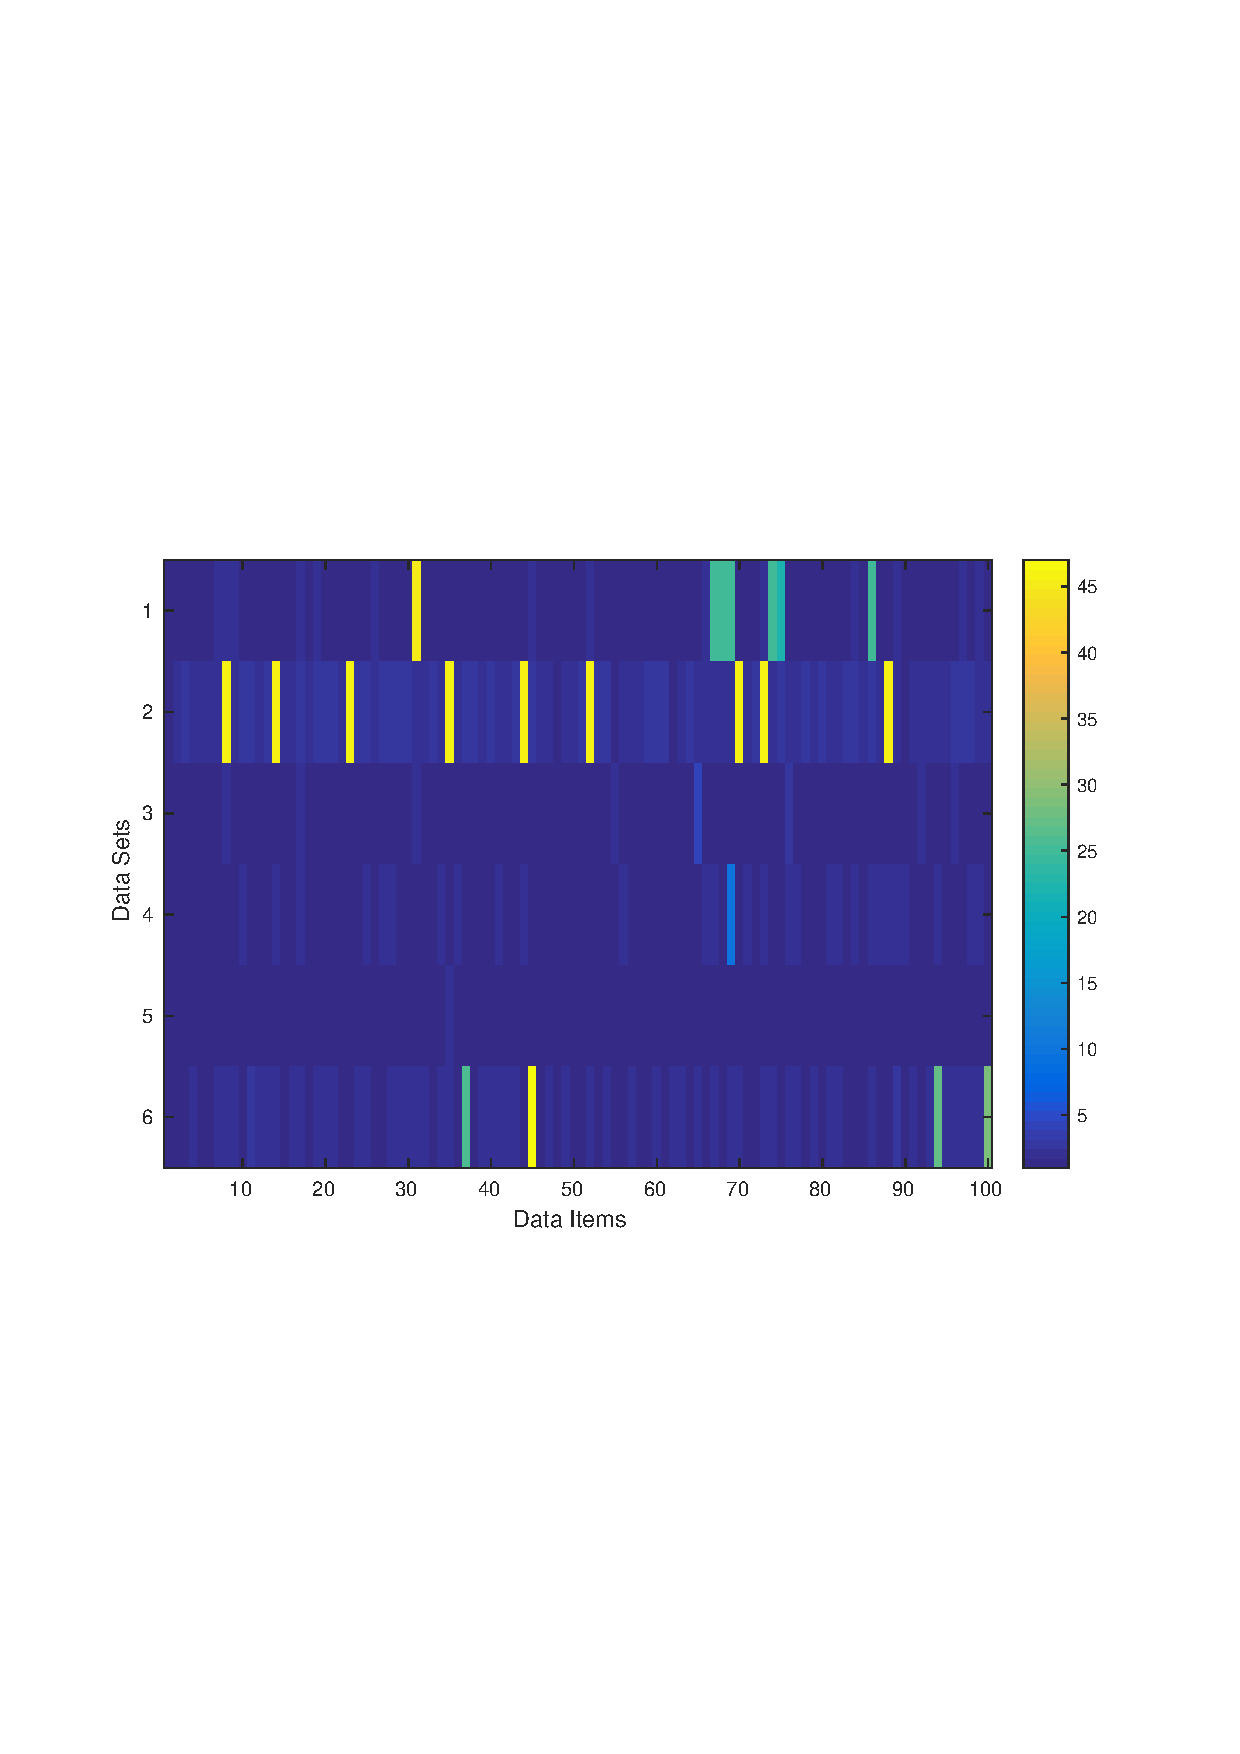
\includegraphics[width=\linewidth]{Plots/mdi_smc_allocations.pdf}
\caption{Results of implementation of SMC within the MDI algorithm}
\label{fig:alloc}
\end{figure}


\bibliography{../Final_report/bibliography.bib}
\bibliographystyle{plain}

\end{document}